\documentclass[output=paper]{langsci/langscibook} 
\author{Kajsa Djärv\affiliation{University of Pennsylvania}\and 
Caroline Heycock\affiliation{University of Edinburgh}\lastand
Hannah Rohde \affiliation{University of Edinburgh}}
\title{Assertion and factivity: Towards explaining restrictions on embedded V2 in Scandinavian} 
\abstract{Since \citet{HooperThompson1973}, many researchers have pursued the insight that V2 is licensed by assertion.  H\&T categorise predicates depending on whether their complement can be asserted: e.g. communication verbs (\emph{say}) permit the assertion of their complement, in contrast to factives (\emph{be happy}). \citet{Simons2007} proposes distinguishing between embedded propositions that do or do not constitute the Main Point of Utterance (MPU) -- a sharpening of the notion of assertion: in question/response-sequences, the proposition answering the question is the MPU. Given this definition/diagnostic for assertion, factives \emph{can}, given the appropriate discourse context, embed MPU and thus should allow embedded V2 (EV2). This paper presents two experiments testing whether factives can embed MPU and whether MPU licenses EV2 in Swedish. The results support both \citegen{Simons2007} contention that factives can embed MPU, while providing new evidence that MPU does not correlate with EV2.}

\ChapterDOI{10.5281/zenodo.1117696}
\maketitle

\begin{document}
\rohead{\thechapter\hspace{0.5em}Assertion and factivity}
\section{Introduction}
%One of the many topics in \ili{Scandinavian} syntax to which Anders Holmberg has made a significant contribution is that of the nature of ``Verb Second''  (V2\is{verb second}); see most recently his survey article, \cite{holmberg13}. REPLACE WITH:

The study of ``Verb Second'' (V2\is{verb second}) has a long history in the literature on \ili{Scandinavian} syntax (see review in \citealt{Holmberg2013}). Although as a first approximation V2\is{verb second} is a phenomenon that is characteristic of root clauses, it has long been known that it occurs also in a restricted set of embedded clauses. What remains unresolved is a precise characterisation -- and a fortiori a theoretical account -- of this restricted distribution in embedded contexts. In this paper we present new experimental results concerning one aspect of the distribution of embedded V2\is{verb second}, namely the constraints on where it can appear in the complement to various types of verb. At issue is whether such cases of V2\is{verb second} are sensitive primarily to local lexical constraints or are reflective of \isi{pragmatic} factors concerning the status of the embedded clause in the larger discourse context.

All the \ili{Scandinavian} languages exhibit V2\is{verb second} robustly in root clauses. Unlike \ili{German} and \ili{Dutch}, they are SVO languages and hence in many subject-initial clauses the V2\is{verb second} property is not unambiguously manifested. If a non-subject occurs in first position in a root clause, however, the finite\is{finiteness} verb must immediately follow it: hence (\ref{ex:denh:1}) is an unambiguous example of a V2\is{verb second} clause in \ili{Swedish}.% page 1 in draft. 

\protectedex{
\ea \label{ex:denh:1}
\gll Den h{\"a}r boken l{\"a}ste han inte.\\
     this  here book.\textsc{def} read he not\\
\glt `This book, he didn't read.' \z
}


%\begin{exe}
%\ex   {\gll Huggormar har jag {\"a}rligt talat aldrig sett i den h{\"a}r skogen.\\
%		adders have I honestly speaking never seen in this here forest.\textsc{def}\\
%		\trans `To be honest, I have never seen adders in this forest.'} \label{huggormar}
%\end{exe}

In the standard varieties of the \ili{Mainland Scandinavian} languages there is an additional diagnostic. In contexts in which V2\is{verb second} is expected not to be found, such as embedded interrogatives or \isi{relative} clauses, sentential \isi{negation} precedes the finite\is{finiteness} verb.\footnote{The difference in this respect between these varieties and \ili{Icelandic} in particular has been intensively researched in a series of independent and collaborative works by Anders Holmberg and Christer Platzack, see e.g.\ \cite{Platzack1987,PlatzackHolmberg1989,HolmbergPlatzack1991,HolmbergPlatzack1995,Holmberg2010parameters}.}   In root clauses, however, the finite\is{finiteness} verb obligatorily precedes \isi{negation}. This contrast is illustrated in (\ref{ex:dethar:2}). 


\protectedex{
\ea\label{ex:dethar:2}
	\ea 
    \gll Det h{\"a}r {\"a}r boken som han \textbf{inte} \textbf{l{\"a}ste}. \\
this here is book.\textsc{def} that he not read\\
\glt `This is the book that he didn't read.'\\
	\ex
    \gll Han \textbf{l{\"a}ste} \textbf{inte} den h{\"a}r boken. \\
he    read not this here book.\textsc{def} \\
\glt `He didn't read this book.'
   \z
	\z} 
%\begin{exe}
%\ex \label{denhar}
%\begin{xlist}
%\ex {\gll Det h{\"a}r {\"a}r boken som han \textbf{inte} \textbf{l{\"a}ste}. \\
 %       this here is book.\textsc{def} that he not read\\
  %      \trans `This is the book that he didn't read.'}
   %     \ex {\gll Han \textbf{l{\"a}ste} \textbf{inte} den h{\"a}r boken. \\
    %           he    read not this here book.\textsc{def} \\
     %    \trans `He didn't read this book'}
%\end{xlist}
%\end{exe}
It is standardly assumed, then, that \isi{negation} in these languages occupies a position above that of the finite\is{finiteness} verb in a non-V2\is{verb second} sentence, but that part of the derivation of V2\is{verb second} involves movement of the verb to a higher position in the left periphery.  Hence the V\textsubscript{fin}$\prec$Neg\is{negation} order is standardly used as a diagnostic for a clause exhibiting V2\is{verb second}.

As just stated, root clauses in \ili{Mainland Scandinavian} contrast with relatives or embedded interrogatives in that these latter contexts disallow V2\is{verb second}. However, as is well-known, in some cases V2\is{verb second} appears to be possible in embedded clauses, as in (\ref{ex:hansaatt}b):

% \protectedex{
\ea\label{ex:hansaatt}	
	\ea 
    \gll Han sa att han \textbf{inte} \textbf{hade} l{\"a}st den h{\"a}r  boken. \\
			he said that he not had read this here book.\textsc{def}\\
	 \glt `He said that he hadn't read this book.' 
	\ex 
    \gll Han sa att han \textbf{hade} \textbf{inte}  l{\"a}st den h{\"a}r  boken. \\
			he said that he  had not read this here book.\textsc{def}\\
         \glt `He said that he hadn't read this book.'         \z   
	\z
% 	}

%\begin{exe}
%\ex \label{hansa}
%\begin{xlist}
%\ex {\gll Han sa att han \textbf{inte} \textbf{hade} l{\"a}st den h{\"a}r  boken. \\
 %       he said that he not had read this here book.\textsc{def}\\
  %      \trans `He said that he hadn't read this book.'}
   %     \ex {\gll Han sa att han \textbf{hade} \textbf{inte}  l{\"a}st den h{\"a}r  boken. \\
%        he said that he  had not read this here book.\textsc{def}\\
 %       \trans `He said that he hadn't read this book.'}        
%\end{xlist}
%\end{exe}
Such examples of embedded Verb Second (EV2) constitute a classic case of an ``Embedded Root Phenomenon,'' and much of the discussion of the distribution of EV2 has relied heavily on the insights of \cite{HooperThompson1973} (H\&T) -- although H\&T discussed only English.  On the one hand, H\&T established five different classes of predicates taking clausal complements, noting in particular that \textbf{factive} predicates did not license \isi{root phenomena} in their complements.\footnote{Here we follow H\&T in our use of “\isi{factive}” and “semifactive”; these two classes are now commonly referred to as “emotive factives\is{factive}” and “cognitive factives\is{factive}” respectively.} On the other, H\&T argued that this constraint on \isi{factive} complements derived ultimately from the impossibility of such complements being \textbf{asserted}; the fundamental claim being that \isi{root phenomena} in general are only possible in assertions, for reasons which H\&T took to be essentially \isi{pragmatic}.  

In work on EV2 in \ili{Scandinavian} ever since \citegen{Andersson1975} classic dissertation, both of these aspects of H\&T's analysis have been invoked. One important {question} is whether H\&T were correct in their argument -- revisited in recent corpus work by \cite{JensenChristensen2013} -- that the (claimed) ungrammaticality of \isi{root phenomena} in \isi{factive} complements is in fact an epiphenomenon, with the ultimate explanation being tied rather to \isi{assertion}.

In this paper we discuss how the work of \cite{Simons2007} 
gives us a way to address this {question}. Simons' concept of ``Main Point of Utterance\is{utterance}'' (MPU\is{Main Point of Utterance}) can be seen as a more precise characterisation of what H\&T refer to as the ``main \isi{assertion}.''  We first provide experimental evidence, using Simons' Question-Answer paradigm, that manipulations of the discourse context can indeed influence what comprehenders take to be the MPU\is{Main Point of Utterance}. We also confirm that embedded clauses, even under factives\is{factive}, can be the MPU\is{Main Point of Utterance} (Experiment 1). Then we test whether that type of manipulation of the discourse context influences the acceptability of EV2 in \ili{Swedish} or whether the acceptability of EV2 is determined solely by the class of the embedding predicate (Experiment 2).  The results show that the acceptability of EV2 is sensitive only to predicate type, with no evidence for \isi{pragmatic} variation dependent on MPU\is{Main Point of Utterance}. The implications of these results are discussed in the final section.
%Alter wording here if we write a ``Conclusion'' after the Discussion section.


\section{The licensing of embedded verb second in Scandinavian}

\subsection{Factivity, presupposition, and assertion}
\label{sec:factivity}

The observation that embedded clauses can have the syntactic properties of root clauses goes back at least to \cite{Emonds1970}, but a central article that has inspired much subsequent work is \cite{HooperThompson1973}. In this study of embedded \isi{root phenomena} in English, H\&T distinguish between five classes of predicates that take clausal complements, as summarised below.  The acceptability of embedded \isi{root phenomena} is argued to reflect these predicate classes, deriving ultimately from the extent to which material in the complement clause can be \textbf{asserted}.\newpage

\begin{description}
\item[Class A predicates] e.g.\ \textit{say}, \textit{report}, \textit{be true}, \textit{be obvious}. The verbs in this group are -- with the possible exception of \textit{vow} -- all verbs of communication, while the adjectives express high degrees of certainty. These predicates can function ``parenthetically'', in which case the subordinate clause has been said to constitute the ``main \isi{assertion}'' of the sentence. H\&T maintain that root transformations are available \textit{iff} the embedded clause consitutes the main \isi{assertion} (p. 477). 
\item[Class B predicates] e.g.\  \textit{suppose}, \textit{expect}, \textit{it seems},  \textit{it appears}. This group contains only verbs, which seem to fall into two subsets: verbs of thought, and impersonals. In this group also the predicates can function parenthetically, in which case the subordinate clause is likewise asserted. Class B predicates in English allow ``Neg\is{negation} raising'' and tag questions based on the subordinate clause.
\item[Class C predicates] e.g.\ \textit{be (un)likely}, \textit{be (im)possible}, \textit{doubt}, \textit{deny}.  H\&T do not offer a general characterization of this class of predicates, but comment that their complements are neither asserted nor presupposed, and that these predicates cannot be used parenthetically. 
\item[Class D predicates] e.g.\ \textit{resent}, \textit{regret}, \textit{be sorry}, \textit{be surprised}, \textit{be interesting}. These are the (emotive) \isi{factive} predicates. Given H\&T's assumptions about the relation between factivity, \isi{presupposition}, and \isi{assertion}, the use of these verbs entails that the complement of these verbs is presupposed, and cannot be asserted.
\item[Class E predicates] e.g. \textit{realize}, \textit{learn}, \textit{discover}, \textit{know}.\footnote{Whether \textit{know} should be grouped together with the semifactives is highly contentious; here we take no position on this.}  This group constitutes the semifactives, which presuppose/entail the truth of their complements only in some environments -- in particular, this \isi{presupposition} can be lost in questions and conditionals \citep{KiparskyKiparsky1970}. 
 
\end{description}

H\&T make the empirical claim that embedded \isi{root phenomena} in English are impossible in the complements of Class C and Class D predicates. They then argue that this follows from the fact that in neither case can the complement be asserted; \isi{assertion} is, on their assumptions, incompatible with \isi{presupposition} (and hence with factivity, since factives\is{factive} presuppose the truth of their complements). Problematically for H\&T's analysis, but as they themselves observe, \isi{root phenomena} in English can occur in the complement to semifactive verbs even in the environments in which they behave like factives\is{factive} (e.g.\ when they occur in non-\is{Modal}modal, declarative contexts). As pointed out in \cite{WiklundEtAl2009}, and as will be discussed further below, the same holds for embedded V2\is{verb second} in \ili{Scandinavian}.  H\&T also claim that for non-\isi{factive} predicates in classes A and B, embedded \isi{root phenomena} are possible if and only if the embedded clause constitutes the \textbf{main assertion} of the sentence. H\&T then argue that \isi{assertion} licenses the \isi{root phenomena} they are investigating in English because all these phenomena involve emphasis, and ``emphasis would be unacceptable in clauses that are not asserted'' (p.\ 472). There are problems for this last link in their argument (for some discussion see e.g.\ \citealt{Heycock2006}).  However, their observation about the absence of \isi{root phenomena} from \isi{factive} complements in particular, and, conversely, the association of such phenomena with some notion of ``\isi{assertion}'' has had a lasting influence.

Despite this, the term ``\isi{assertion}'' itself has largely been abandoned in recent literature. As \citet[1041]{SimonsEtAl2010} points out, the point of clause embedding is often precisely to indicate the weakness of the speaker's commitment to the proposition expressed, whereas \isi{assertion} is generally taken to involve a strong commitment. Observe, for example,  the lower speaker commitment conveyed in (\ref{ex:ibelieve}) compared to (\ref{ex:itwill}):  

\protectedex{
	\ea\label{ex:ibelieve} I believe that it will rain tomorrow.  \z
	\ea\label{ex:itwill} It will rain tomorrow.  \z}
%\begin{exe}
%	\ex I believe that it will rain tomorrow.  \label{ibelieve}
%	\ex It will rain tomorrow. \label{itwill}
%\end{exe}

Still, we want to capture the intuition that in (\ref{ex:ibelieve}), the main proposition conveyed by the speaker is typically the proposition that it will rain tomorrow (and not that the speaker has a belief about the rain tomorrow). \cite{Simons2007} introduces the concept ``Main Point of Utterance\is{utterance}'' (MPU\is{Main Point of Utterance}) for this purpose.\footnote{We will keep to the convention of referring to verbs of communication and cognition such as \textit{say}, \textit{claim} and \textit{think}, which generally accept MPU-complements, as ``assertive''. However, we will use the term MPU\is{Main Point of Utterance}, rather than ``\isi{assertion}'', when referring to the discourse status of the proposition expressed by the embedded clause. } She provides the following working definition of MPU\is{Main Point of Utterance}:

\begin{quote}
	[T]he main point of an \isi{utterance} U of a declarative sentence S is the proposition p, communicated by U, which renders U relevant. [ \ldots\ ] To sharpen intuitive judgments, we will utilize \isi{question}/response sequences as a diagnostic for main point content. I assume that whatever proposition communicated by the response constitutes an answer (complete or partial) to the \isi{question} is the main point of the response. \citep[1035--1036]{Simons2007}
\end{quote}

This definition provides a useful tool for identifying the MPU\is{Main Point of Utterance} in an \isi{utterance}. Importantly, it makes MPU\is{Main Point of Utterance} a property relative to a discourse, rather than to a sentence, as illustrated in (\ref{ex:whydidntkate}) and (\ref{ex:whydidntjohn}):

\protectedex{
	\ea\label{ex:whydidntkate} \begin{itemize}
		\item[Q.] Why didn't Kate come to the party?
		\item[A.] John thinks that she's left town.
	\end{itemize} \z 
	\ea \label{ex:whydidntjohn} \begin{itemize}
		\item[Q.] Why didn't John invite Kate to the party?
		\item[A.] He thinks that she's left town.
	\end{itemize} \z }

%\begin{exe}
%	\ex \begin{itemize}
%		\item[Q.] Why didn't Kate come to the party?
%		\item[A.] John thinks that she's left town.
%	\end{itemize}  \label{whydidnt1}
%	\ex \label{whydidnt2}\begin{itemize}
%		\item[Q.] Why didn't John invite Kate to the party?
%		\item[A.] He thinks that she's left town.
%	\end{itemize}
%\end{exe}

(\ref{ex:whydidntkate}-A) and (\ref{ex:whydidntjohn}-A) are formally identical, expressing the proposition that John thinks that Kate has left town. Where they differ is precisely at the level of MPU\is{Main Point of Utterance}. Following \citet[1037]{Simons2007}  (\ref{ex:whydidntkate}-A) can be paraphrased as ``The answer to your \isi{question} why Kate didn't come to the party may be that she has left town. I'm saying this based on what John told me that he believes to be the case.'', and (\ref{ex:whydidntjohn}-A) as ``The answer to your \isi{question} why John didn't invite Kate to the party is that he thinks that she was out of town and therefore would be unable to attend.'' In (\ref{ex:whydidntkate}-A), the root clause \textit{John thinks} has a parenthetical, essentially evidential use, qualifying the speaker's claim that Kate is out of town.\footnote{The observation that embedding verbs can be used parenthetically is originally due to \citet[484]{Urmson1952} who explains the parenthetical use as ``priming the hearer to the emotional significance, the logical relevance, and the reliability of our statements.''} 

We now return to the \isi{question} of why some, but not other predicates appear to be felicitous when used with this discourse function. Compare, for example, (\ref{ex:whendoes1}) and (\ref{ex:whendoes2}):

\protectedex{
	\ea\label{ex:whendoes1}
		\ea When does the game start? 
        \ex I think that it starts at 10.
        \z
 \z }

\protectedex{
	\ea\label{ex:whendoes2}
    \ea When does the game start?
	\ex I know that it starts at 10.
	\ex I'm happy that it starts at 10. 
    \ex I regret that it starts at 10.
    \z
	\z }

%\begin{exe}
%	\ex \label{whendoes1}
%	\begin{xlist}
%		\ex When does the game start?
%		\ex I think that it starts at 10. 
%	\end{xlist}
%	\ex \label{whendoes2}
%	\begin{xlist}
%		\ex {When does the game start?}
%		\ex[\#]{I know that it starts at 10.} 
%		\ex[\#]{I'm happy that it starts at 10.}
%		\ex[\#]{I regret that it starts at 10.}
%	\end{xlist}
%\end{exe}

As discussed above, according to \citet{HooperThompson1973} and \citet{Hooper1975},\linebreak clause-embedding factives\is{factive} (such as \textit{be happy} and possibly \textit{know}) cannot be used parenthetically in this way,  that is, with the main \isi{assertion} being the embedded clause. They take this to be because the \isi{factive} predicate \textbf{presupposes} the embedded proposition. That is, the embedded proposition is taken to be part of the conversational common ground, and therefore cannot be used to update the common ground (by adding propositions to it, in the sense of  \citealt{Stalnaker1974}, \citeyear{Stalnaker2002}). In essence, this is to claim that a \isi{factive} complement cannot be the MPU\is{Main Point of Utterance}. Interestingly however, as already mentioned, \citet{HooperThompson1973} note that semifactives, which can lose their factivity in questions and in the antecedents of conditionals, \textit{can} be used parenthetically even in contexts where their factivity is retained.  H\&T demonstrate this by showing that, for example, a tag \isi{question} can be formed from the complement to such a verb, which they take to indicate that this complement is the main \isi{assertion}; they contrast this with the behaviour of a true \isi{factive}. The following examples are H\&T's examples (129) and (131): %p. 481

\protectedex{
	\ea \label{ex:tag} 
		\langinfo{}{}{\citealt[481]{HooperThompson1973}}
	
	I see that Harry drank all the beer, didn't he? 
	\z}
	
\protectedex{
	\ea \label{ex:tagstar}  
		\langinfo{}{}{\citealt[481]{HooperThompson1973}}

	{*I am sorry that Suzanne isn't here, is she?} 
	\z }
%\begin{exe}
%\ex[] {I see that Harry drank all the beer, didn't he?}
%\ex [*] {I am sorry that Suzanne isn't here, is she?}
%\end{exe}

\noindent \cite{Simons2007} makes the same point by demonstrating that the complement to a semifactive like \textit{discover} can constitute the MPU\is{Main Point of Utterance}. The following is her example (21a): % p. 1045

\protectedex{
\ea\label{ex:wheredid} 
	\langinfo{}{}{\citealt[1045]{Simons2007}}

	\begin{itemize}
		\item[Q: ] Where did Louise go last week?
		\item[A: ] Henry discovered that she had a job interview at Princeton.
       \end{itemize} \z }
%\begin{exe} 
%	\ex \begin{itemize}
%		\item[Q: ] Where did Louise go last week?
%		\item[A: ] Henry discovered that she had a job interview at Princeton.
%	\end{itemize} \label{wheredid}
%\end{exe}
Simons' conclusion %, shared with a \isi{number} of authors,
%Q - Kajsa - do you have refs?
is that semifactives show us that \isi{presupposition} and factivity must be disassociated. Presuppositions are treated by the speaker as part of the conversational common ground. In contrast, factivity is the entailment of the truth of the embedded proposition. For parenthetical assertives, like \textit{think} or \textit{say}, the complement is neither presupposed nor entailed.  In (\ref{ex:wheredid}-A) on the other hand, the complement is entailed (Henry could not have discovered that Louise had a job interview at Princeton unless she did in fact have such an interview), but it is not presupposed. That is, it provides discourse-new information, serving the function of updating the conversational common ground (it is the MPU\is{Main Point of Utterance}).

A \isi{question} that naturally arises from this observation is the following: if factivity does not block MPU\is{Main Point of Utterance} (that is, if factivity does not entail \isi{presupposition}), why is it that \textit{true} factives\is{factive} (like \textit{know}, \textit{regret} and \textit{be happy}), unlike semifactives (like \textit{discover} and \textit{realize}) resist MPU-complements, as exemplified by the infelicity of (\ref{ex:whendoes2}d)? In other words, what is it about factives\is{factive}, that is not the property of factivity itself, that render these infelicitous as parentheticals? A plausible answer to this {question} comes from \citet{Simons2007}. She appeals to what is an essentially Gricean reasoning process to explain how parenthetical uses of embedding predicates come about. In (\ref{ex:theresponse}) we sketch an outline of the \isi{pragmatic} process which, according to these authors, underlies the parenthetical use of \textit{think} in (\ref{ex:whydidntkate}) above.

\protectedex{
	\ea\label{ex:theresponse}
	\begin{itemize}
	\item The response to the \isi{question} ``Why didn't Kate come to the party?'' in (\ref{ex:whydidntkate}) contains two propositions, \textit{p}: \emph{John thinks \textit{q}}, and \textit{q}: \emph{Kate has left town}. Only \textit{q} directly answers this \isi{question}. 
	\item Assuming that the speaker is being cooperative, and intends to answer the \isi{question} in a conversationally appropriate manner (given Quantity\is{maxim of quantity}, Relevance etc.), the hearer infers that the speaker must have some reason for not directly asserting \textit{q}. Such a reason could be that she does not have sufficient evidence for directly asserting \textit{q}. However, \textit{p}, indicating that John is the source of \textit{q}, allows the speaker to offer \textit{q} as a possible answer to the \isi{question}.
	\end{itemize}
	\z }
%\begin{exe}
%	\ex\label{theresponse}
%	\begin{xlist}
%		\ex The response to the \isi{question} ``Why didn't Kate come to the party?'' in (\ref{whydidnt1}) contains two propositions, \textit{p}: \emph{John thinks \textit{q}}, and \textit{q}: \emph{Kate has left town}. Only \textit{q} directly answers this \isi{question}.
%		\ex Assuming that the speaker is being cooperative, and intends to answer the \isi{question} in a conversationally appropriate manner (given Quantity\is{maxim of quantity}, Relevance etc.), the hearer infers that the speaker must have some reason for not directly asserting \textit{q}. Such a reason could be that she does not have sufficient evidence for directly asserting \textit{q}. However, \textit{p}, indicating that John is the source of \textit{q}, allows the speaker to offer \textit{q} as a possible answer to the \isi{question}.
%	\end{xlist} 
%\end{exe}

The restriction on factives\is{factive} as parentheticals now follows quite naturally \citep[1049-1050]{Simons2007}. The following is from her example (37):% p. 1050

\protectedex{
	\ea\label{ex:whydidntlouise} 
	\langinfo{}{}{\citealt[1050]{Simons2007}}
     \ea Where did Louise go yesterday?
	 \ex Henry forgot that she went to Princeton. 
	  \ex Henry remembered that she went to Princeton. 
	%	\ea[\#]{It's odd that she went to Princeton.}
    \z
	\z }
%\begin{exe}
%	\ex \begin{xlist}
%		\ex[] {Where did Louise go yesterday?}
%		\ex[\#]{Henry forgot that she went to Princeton.}
%		\ex[\#]{Henry remembered that she went to Princeton.}
%		%	\ex[\#]{It's odd that she went to Princeton.}
%	\end{xlist} \label{whydidnt3}
%\end{exe}
As shown in (\ref{ex:whydidntlouise}), these matrix clauses are problematic as parentheticals. %It is not clear how Henry's forgetting or  remembering that Kate has left town is relevant to the \isi{question} just asked. REPLACE WITH:
It is not clear how Henry's forgetting or remembering that Kate has left town is relevant to the \isi{question} just asked (though see example (\ref{ex:sorry}) for a \isi{question} that makes such information relevant). The responses thus present a violation of \citegen{Grice1975} Maxim of Quantity\is{maxim of quantity}, in that they provide the hearer with considerably more information than the \isi{question} asked for. Further, consider the case of \textit{know}. The following is from \citegen{Simons2007} example (35): %p. 1049

\protectedex{
		\ea\label{ex:wherewas2} 
	\langinfo{}{}{\citealt[1049]{Simons2007}}
		\ea Where was Louise yesterday?
		\ex ??Henry knows that she was in Princeton.
        \z
	\z }

%\begin{exe}
%	\ex \begin{xlist}
%		\ex[] {Where was Louise yesterday?}
%		\ex[??]{Henry knows that she was in Princeton.}
%	\end{xlist} \label{wherewas2}
%\end{exe}

The meaning of \textit{know} is essentially to express a strong commitment to the truth of its complement. However, this is also the function of directly asserting the proposition. Hence, it is not clear what non-redundant discourse function would be achieved by embedding the proposition under \textit{know}. In effect then, it is not the factivity \textit{per se} that renders the \isi{utterance} bad, but rather the lack of relevant communicative content contributed by the matrix clause. 

This point can be further illustrated with an ``assertive'' matrix predicate. Imagine someone blurting out, out of the blue:

\protectedex{
	\ea\label{ex:isay} I say that I will go and get a coffee. \z }
%\begin{exe}
%	\ex I say that I will go and get a coffee. \label{isay}
%\end{exe}

A hearer might wonder what the purpose of the embedding is, given that the matrix clause does not fill any clear conversational purpose beyond what would be accomplished simply by asserting ``I will go and get a coffee.'' However, given an appropriate discourse context, factives\is{factive} like \textit{know} and \textit{forget} can be assigned felicitous parenthetical readings. The following examples are \citegen{Simons2007} (36) and (39):\footnote{Note also that with appropriate stress placement, a sentence like ``I know that she's in \textit{Princeton}'' and a continuation like ``...but I don't know if that answers your \isi{question}?'', would render \textit{know} much more natural in answering a \isi{question} like (\ref{ex:wherewas2}) (see \citealt[1049]{Simons2007}).} %example, p. 1050

\protectedex{
	\ea\label{ex:wherewas} 
	\langinfo{}{}{\citealt[1050]{Simons2007}}
	
	\begin{itemize}
		\item[Q: ] Where was Louise yesterday?
		\item[A: ] Y'know she had to go to Princeton.
	\end{itemize} \z }

\protectedex{
	\ea\label{ex:sorry} 
	\langinfo{}{}{\citealt[1050]{Simons2007}}

	Sorry, we're going to have to change our plans for dinner tonight.

		\ea Henry forgot that he has an evening appointment.
		\ex Henry just realized/remembered that he has an evening appointment.
        \z
	\z }

%\begin{exe}
%	\ex \begin{itemize}
%		\item[Q: ] Where was Louise yesterday?
%		\item[A: ] Y'know she had to go to Princeton.
%	\end{itemize} \label{wherewas}
%	\ex  Sorry, we're going to have to change our plans for dinner tonight.
%	\begin{xlist}
%		\ex Henry forgot that he has an evening appointment.
%		\ex Henry just realized/remembered that he has an evening appointment.
%	\end{xlist} \label{sorry}
%\end{exe}

In (\ref{ex:wherewas}), \textit{know} fills a non-evidential parenthetical function. Roughly,\largerpage the answer can be paraphrased as ``Louise had to go to Princeton yesterday, and you know that already (so you shouldn't be asking).'' (Compare with a slightly modified version of (16): ``I said that I will go and get a coffee!'' whereby the embedding is understandable and non-redundant if the speaker is trying to highlight that the hearer was not listening.)
%(Compare with a slightly modified version of (\ref{isay}): ``I said that I will go and get a coffee!'') REPLACE WITH:
In (\ref{ex:sorry}a,b) on the other hand, the speaker is citing Henry's evening appointment as the reason for changing the dinner plans. Here, \textit{forget/realize/remember}  fill the relevant discourse function of informing the hearer of the reason for not telling her earlier. \citeauthor{Simons2007} uses examples like (\ref{ex:wherewas}) and (\ref{ex:sorry}) to support her claim that a \isi{factive} can function parenthetically in an appropriate discourse context, such that its embedded clause acts as the main \isi{assertion}. Our first study tests this claim experimentally.

\subsection{(Non)factivity or MPU as a factor for embedded verb second}\label{nonfactivityOrMPU}

We have summarised above aspects of the proposal in \cite{Simons2007}, according to which H\&T's concept of ``main \isi{assertion}'' is replaced by that of ``Main Point of Utterance\is{utterance},'' and MPU\is{Main Point of Utterance} in turn is argued to be a conversational property of utterances in context, sensitive both to properties of the discourse, as well as to a number of linguistic factors that we have not discussed here.  As shown above, under this view -- in contrast to that of H\&T -- factivity is not incompatible with MPU\is{Main Point of Utterance} status.  %While neither H\&T nor Simons discuss data from any language other than English, there is a tradition that dates back at least as far as \cite{andersson75}  of taking Embedded Verb Second (EV2) in \ili{Scandinavian} to be another type of ``Embedded Root Phenomenon,'' whose distribution can be analysed along the lines set out in H\&T.  REPLACE WITH:
While neither H\&T nor \citeauthor{Simons2007} discuss data from any language other than English, there is a tradition that dates back at least as far as \citet{Andersson1975} of taking Embedded Verb Second (EV2) in \ili{Scandinavian} to be another type of ``Embedded Root Phenomenon".  EV2 is known to be sensitive to a variety of factors (see e.g., \citealt{Zwart1997}), but of interest here is how its distribution can be analysed along the lines set out in H\&T. Given Simons' argument that the lexical semantic\is{semantics} property of (non-)factivity can be teased apart from the discourse \isi{pragmatic} property of being the MPU\is{Main Point of Utterance},  the {question} evidently arises as to which of these is relevant to the licensing of EV2.

Clearly, one possible hypothesis is that the crucial concept for the distribution of EV2 in \ili{Scandinavian} is MPU\is{Main Point of Utterance}, and that any apparent association with non-factivity is due to the greater ease -- given the interaction between lexical meaning and discourse contexts -- with which non-\isi{factive} verbs can embed the MPU\is{Main Point of Utterance}. This hypothesis is put forward explicitly in \cite{JensenChristensen2013}, a corpus study of EV2 in \ili{Danish}.\ \cite{JensenChristensen2013} state as their hypothesis that 
``V\textgreater Adv [EV2 order] signals foregrounding of the subordinate clause, i.e.\ that its content is the main point of the \isi{utterance}.''  However, they do not code for MPU\is{Main Point of Utterance} in any direct way, while they do code for (among other factors)  the ``type of the matrix predicate,'' described as an operationalization of H\&T's five classes of predicates, with the addition of   a class of ``Causatives'' and a residual ``Other'' class.\footnote{H\&T's Class C was not coded for as it turned out there were virtually no tokens of this class in their corpus (p. 50).}   They discover a clear effect of predicate type, but interpret it as supporting their MPU\is{Main Point of Utterance} hypothesis (note that they intend their use of ``foreground'' to mean the same as MPU\is{Main Point of Utterance} (p.~40)):
\begin{quotation}
\noindent [ \ldots ] both \textsc{Factive} and \textsc{Causative} matrix predicates, \textit{as expected from the hypothesis of V\textgreater Adv as a foregrounding signal} [our emphasis], clearly disfavour V\textgreater Adv word order [ \ldots ] Subclauses governed by communicative predicates [Class A] are significantly more disposed to V\textgreater Adv word order than subclauses governed by cognitive predicates [Class B], which are again significantly more disposed to V\textgreater Adv than \textsc{Other} predicates. \textit{This, again, supports the hypothesis of V\textgreater Adv as a foregrounding signal, since we would expect communicative predicates to frequently govern subclauses that are foregrounded}, [our emphasis]  even when they do not contain any explicit signals of being quotes   [ \ldots ] Cognitive predicates will often introduce something important that the speaker or some other {person} knows or has learned, \textit{and these would then be foregrounded} [our emphasis]. \citep[50]{JensenChristensen2013}
\end{quotation}
So while their hypothesis is clearly that EV2 (or at least, the V\textgreater Adv order that we take to be one manifestation of this structure) is a signal of MPU\is{Main Point of Utterance}, they in fact have only indirect evidence for this (essentially as was the case also for H\&T).

Another author who could be read as adopting the hypothesis that MPU\is{Main Point of Utterance} is the crucial concept for licensing EV2 in \ili{Scandinavian} is \citet{Julien2009,Julien2015}, 
although this is less clear. In both papers \citeauthor{Julien2009} argues that EV2 signals \isi{assertion}, but it is not always clear how \isi{assertion} is defined (and hence diagnosed). As a result the extent to which her understanding of this might differ from Simon's definition of MPU\is{Main Point of Utterance} is not always clear. In \cite{Julien2009} the term MPU\is{Main Point of Utterance} is never used, and Simons' work is not referenced; in \cite{Julien2015} she argues explicitly against the relevance of MPU\is{Main Point of Utterance}, although her argument mainly bears on the particular use of the concept in \cite{WiklundEtAl2009}, to be discussed shortly.\footnote{  
One important aspect of \citeauthor{Julien2009}'s proposal which does clearly distinguish it from one which links EV2 exclusively to MPU\is{Main Point of Utterance} status (as for example is the case in \citealt{JensenChristensen2013}) is that she essentially allows for two ways in which EV2 might be licensed. On the one hand, a clause with EV2 may be a ``direct \isi{assertion},'' that is, one attributed to the speaker. This comes very close to -- or is perhaps identical to -- the concept of the embedding predicate having an evidential, parenthetical interpretation (see the discussion in Section~\ref{sec:factivity} above). On the other, a clause with EV2 may be the report of an \isi{assertion} made by the {person} denoted by the subject of the embedding verb. This predicts that EV2 would be possible in a context like the following, for example, where the \citet{JensenChristensen2013} hypothesis would exclude it, since the embedded proposition -- that the world is not round -- can be taken to be an \isi{assertion} of Jasper's, but is clearly not intended to be added to the common ground by the speaker:
\protectedex{
\begin{itemize}
\item[Q: ] Why do you think Jasper isn't so bright?
\item[A: ] He said that the world is not round.  What an idiot!
\end{itemize} }}

One possible hypothesis, then, is that EV2 is directly licensed by, or signals, MPU\is{Main Point of Utterance} status -- a status that under the account of \citet{Simons2007}  is determined relative to a discourse. The alternative is that lexical semantic\is{semantics} properties of the embedding predicates -- (non)-factivity being at least one such property -- are directly responsible for the possibility of EV2 in the embedded clause. A version of this alternative hypothesis can be found in \citet{WiklundEtAl2009}.  
Using the predicate classes identified by H\&T, and taking as their data their own judgments (supplemented in some cases with those of a small number of other linguists), rather than a corpus,  \citet{WiklundEtAl2009} argue that EV2 is grammatical under assertives (Classes A and B) and semifactives (Class E), but not under factives\is{factive} (Class D) or the class of non-assertive, non-presuppositional predicates (Class C). % (2009: 4-9).  Don't think we need to give page numbers for this.
Examples below are from \cite[1918--1921]{WiklundEtAl2009}.

\protectedex{
\ea 
	\langinfo{}{}{\citealt[1918--1921]{WiklundEtAl2009}}

	\gll Han sa att han \textbf{kunde} \textbf{inte} sjunga p{\aa} br\"ollopet.\\
		he said that he could not sing at wedding.\textsc{def}\\
		\glt `He said that he could not sing at the wedding.'\hfill Assertive Class A \z

\ea 
	\langinfo{}{}{\citealt[1918-1921]{WiklundEtAl2009}}
	
	\gll Han trodde att vi \textbf{hade} \textbf{inte} sett den h\"ar filmen. \\
	he believed that we had not seen this here film.\textsc{def}\\
	\glt `He believed that we hadn't seen this film.'\hfill Assertive Class B \z

\ea 
	\langinfo{}{}{\citealt[1918-1921]{WiklundEtAl2009}}

	\gll *Han tvivlar p{\aa} att hon \textbf{har} \textbf{inte} tr\"affat den h\"ar mannen. \\
	he doubts on that she has not met this here man.\textsc{def}\\
	\glt `He doubts that she hasn't met this man.'\hfill Non-assertive Class C	 \z
\ea 
	\langinfo{}{}{\citealt[1918-1921]{WiklundEtAl2009}}

	\gll *Han {\aa}ngrade att han \textbf{hade} \textbf{inte} sjungit.\\
		he regretted that he had not sung.\\
		\glt `He regretted that he hadn't sung.'\hfill \isi{Factive}\is{factive} Class D \z
\ea 
	\langinfo{}{}{\citealt[1918-1921]{WiklundEtAl2009}}

	\gll Jag uppt\"ackte att jag \textbf{hade} \textbf{inte} l\"ast den.\\
		I discovered that I had not read it.\\
	\glt `I discovered that I hadn't read it.'\hfill Semifactive Class E 	\z }

%\begin{exe}
%	\ex[] {\gll Han sa att han \textbf{kunde} \textbf{inte} sjunga p{\aa} br\"ollopet.\\
%		he said that he could not sing at wedding.\textsc{def}\\
%		\trans `He said that he could not sing at the wedding.'\hfill Assertive Class A}
%	\ex[] {\gll Han trodde att vi \textbf{hade} \textbf{inte} sett den h\"ar filmen. \\
%		he believed that we had not seen this here film.\textsc{def}\\
%		\trans `He believed that we hadn't seen this film.'\hfill Assertive Class B}
%	\ex[*] {\gll Han tvivlar p{\aa} att hon \textbf{har} \textbf{inte} tr\"affat den h\"ar mannen. \\
%		he doubts on that she has not met this here man.\textsc{def}\\
%		\trans `He doubts that she hasn't met this man.'\hfill Non-assertive Class C}	
%	\ex[*] {\gll Han {\aa}ngrade att han \textbf{hade} \textbf{inte} sjungit.\\
%		he regretted that he had not sung.\\
%		\trans `He regretted that he hadn't sung.'\hfill \isi{Factive}\is{factive} Class D }
%	\ex[] {\gll Jag uppt\"ackte att jag \textbf{hade} \textbf{inte} l\"ast den.\\
%		I discovered that I had not read it.\\
%		\trans `I discovered that I hadn't read it.'\hfill Semifactive Class E }	
%\end{exe}
Given that EV2 is possible under semifactives -- crucially, even in contexts where their factivity is preserved -- factivity cannot be what restricts the availability of EV2. \citet[14]{WiklundEtAl2009} invoke instead the concept of MPU\is{Main Point of Utterance} from Simons' work. However, this does not mean that they claim that MPU\is{Main Point of Utterance} status is what licenses or is signalled by EV2. First,  while they follow \citet{Simons2007} in that they take MPU\is{Main Point of Utterance} to be the proposition in an \isi{utterance} which is used to update the common ground, and which can be diagnosed by the \isi{question}/answer-pairs discussed above, their understanding of MPU\is{Main Point of Utterance} is in fact crucially different from that of \citet{Simons2007}. They state:

\begin{quote}
Those \textit{predicate classes} [our emphasis] which may not embed an MPU\is{Main Point of Utterance} are exactly those that impose restrictions on V2\is{verb second} in the embedded clause (Class C and D). In other words, MPU-compatible environments correspond to environments where V2\is{verb second} is unrestricted in all four varieties of \ili{Scandinavian} investigated here. \citep[1927]{WiklundEtAl2009} 
\end{quote}\newpage

That is to say, whereas \citeauthor{Simons2007} argues that MPU\is{Main Point of Utterance} is a property of utterances, not predicates, \citeauthor{WiklundEtAl2009} take possible environments for MPU\is{Main Point of Utterance} to be lexically defined, in that MPU\is{Main Point of Utterance} is licensed by assertives and semifactives, but not by factives\is{factive}. 

The second way in which the approach of \citet{WiklundEtAl2009} departs from an account that really depends on the notion of MPU\is{Main Point of Utterance} is that they state clearly that the relation between MPU\is{Main Point of Utterance} and EV2 is only indirect. That is, EV2 and MPU\is{Main Point of Utterance} are licensed in the same structural domain -- ForceP -- that is selected by assertives and semifactives, but not by factives\is{factive}, which select a smaller clause, incompatible with both EV2 and MPU\is{Main Point of Utterance} (2009: 1930). However, they argue that verb-movement and interpretation as MPU\is{Main Point of Utterance} are both optional, and independent, properties of ForceP: hence it is possible for an MPU-clause to be V-in situ (EV3), and for an EV2-clause to not be the MPU\is{Main Point of Utterance}. This much weaker linkage between the two is motivated by the following type of judgments \citep[1927]{WiklundEtAl2009}:


\ea\label{ex:varforkom} 
	

	Varf\"or kom han inte p{\aa} m\"otet ig{\aa}r?\\
	`Why didn't he come to the meeting yesterday?'\\

	\ea  Vi uppt\"ackte att han \textbf{hade} tyv\"arr \textbf{inte} f{\aa}tt p{\aa} vinterd\"acken \"annu.\\ 
	 we discovered that he had unfortunately not put on winter-tires.\textsc{def} yet
	\ex  Vi uppt\"ackte att han tyv\"arr \textbf{inte} \textbf{hade} f{\aa}tt p{\aa} vinterd\"acken \"annu.\\ 
	we discovered that he unfortunately not had put on winter-tires.\textsc{def} yet \\
	 `We discovered that he unfortunately hadn't changed to winter tires yet.' \\
    \citep[1927]{WiklundEtAl2009}
    \z
\z

%\begin{exe}
%	\ex Varf\"or kom han inte p{\aa} m\"otet ig{\aa}r?\\
%	`Why didn't he come to the meeting yesterday?' \label{varforkom}
%	\begin{xlist}
%		\ex \gll Vi uppt\"ackte att han \textbf{hade} tyv\"arr \textbf{inte} f{\aa}tt p{\aa} vinterd\"acken \"annu.\\ 
%		we discovered that he had unfortunately not put on winter-tires.\textsc{def} yet\\ 
%		% Their actual example of EV2:
%		%\ex \gll Vi uppt\"ackte att tyv\"arr \textbf{hade} han \textbf{inte} f{\aa}tt p{\aa} vinterd\"acken \"annu.\\ 
%		%we discovered that he had unfortunately not put on winter-tires.\textsc{def} yet\\  
%		\ex \gll Vi uppt\"ackte att han tyv\"arr \textbf{inte} \textbf{hade} f{\aa}tt p{\aa} vinterd\"acken \"annu.\\ 
%		we discovered that he unfortunately not had put on winter-tires.\textsc{def} yet \\
%		\trans `We discovered that he unfortunately hadn't changed to winter tires yet.' 
%	\end{xlist}
%\end{exe}

They argue that since both (\ref{ex:varforkom}a) and (\ref{ex:varforkom}b) are possible in response to the \isi{question} -- which provides a context that makes the embedded clause in the answer the most plausible MPU\is{Main Point of Utterance} -- it must be the case that MPU\is{Main Point of Utterance} does not require EV2 syntax. Conversely, they also cite examples where the MPU\is{Main Point of Utterance} is \emph{not} the embedded clause, but EV2 is still possible, so there is not even a one-way implication:

\protectedex{

\ea\label{ex:varforkopte}
	

	\ea  Varf\"or kom han inte p{\aa} festen? \\
          why came he not to party.\textsc{def} \\
          `Why didn't he come to the party?' 

	\ex Kristine sa att han \textbf{fick} \textbf{inte}. \\
         Kristine said that he was-allowed not\\
         `Kristine said that he wasn't allowed to.' \\
         \citep[1929]{WiklundEtAl2009}
         \z
\z }
%\begin{exe}
%	\ex \label{varforkopte}
%	\begin{xlist}
%		\ex \gll  Varf\"or kom han inte p{\aa} festen? \\
%		why came he not to party.\textsc{def} \\
%		\trans `Why didn't he come to the party?'
%		\ex \gll Kristine sa att han \textbf{fick} \textbf{inte}. \\
%		Kristine said that he was-allowed not\\
%		\trans `Kristine said that he wasn't allowed to.'\hfill \cite[p.~1929]{wiklund-etal09}
%	\end{xlist}
%\end{exe}

According to \citet[1929]{WiklundEtAl2009}, the answer in (\ref{ex:varforkopte}b) is ambiguous; crucially, it can have the interpretation that one reason for the {person} in {question} not coming to the party was that Kristine said something -- that is, a reading where the MPU\is{Main Point of Utterance} is not the embedded clause, even though this unambiguously displays EV2 word order.

For these reasons, even though \citet{WiklundEtAl2009} explicitly invoke \citeauthor{Simons2007}´ work, in fact the concept of MPU\is{Main Point of Utterance} as presented there plays no explanatory role within their hypothesis; rather, their approach predicts that the possibility -- but not the presence in any given example -- of EV2 is determined by the lexical class of the embedding predicate. 

%\subsubsection{Julien 2009}
%
%A alternative view is offered by Julien (2009).\footnote{She uses the term \textsc{assertion}. However, the \isi{pragmatic} notion relevant to EV2 in her view is essentially the same as Simons' (2007) MPU\is{Main Point of Utterance}. Hence, for terminological consistency, we use the term MPU\is{Main Point of Utterance} here as well.} She argues that embedded EV2 is possible in an embedded clause iff. it is the MPU\is{Main Point of Utterance}, independently of embedding predicate. As for Wiklund \textit{et} al., Julien (2009: 31-32) argues that MPU\is{Main Point of Utterance} is encoded in a ForceP. Unlike the former however, Julien hypothesizes that \isi{Force}^{o} has a uFIN feature, which attracts \textbf{(\isi{EPP}?)} the finite\is{finiteness} verb. Julien would therefore predict that only (20b) is available in response to (20a). As support for her hypothesis, she looks at embedded declaratives in \ili{Swedish}, \ili{Norwegian} and \ili{Danish} corpora (2009: 7-14)\footnote{NoTa. Tagged \ili{Norwegian} corpus, spoken language, approximately 1 million words. The Text Laboratory, University of Oslo. URL: http://www.tekstlab.uio.no/nota/oslo/index.html; The Oslo Corpus of Tagged \ili{Norwegian} Texts, Nynorsk section. Tagged \ili{Norwegian} corpus, written language, apx. 18.5 million words. The Text Laboratory, University of Oslo. URL: http://www.tekstlab.uio.no/norsk/nynorsk/index.html; PAROLE. Tagged \ili{Swedish} corpus, written language, apx. 19 million words. \ili{Swedish} Language Bank, G\"oteborg University. URL: http://spraakbanken.gu.se/parole/; KorpusDK: Tagged \ili{Danish} corpus, written language, apx. 56 million words. Det Danske Spog- og Litteraturselskab. URL: http://ordnet.du/korpusdk.} where she finds instances of EV2 embedded under factives\is{factive} (example from Julien 2009: 11):
%
%\begin{exe}
%\ex \gll Alltid glemte de at den gutten \textbf{var} ikke som andre. \\
%	always forgot they that that boy.def was not like others\\
%	\trans `They always forgot that that boy was not like others.' \hfill \ili{Norwegian} Bokm{\aa}l
%\end{exe}
%
%Although examples like (21) appear to challenge Wiklund \textit{et} al's analysis, it is nonetheless true that Julien finds considerably fewer instances of EV2 under factives\is{factive} than under assertives and semifactives. A different corpus study, by Jensen \& Christensen (2011)\footnote{The LANCHART word-order tudy: The data comes from 132 recordings of 92 \ili{Danish} speakrs in Copenhagen and the village Vinderup in western Jutland, conducted in 1986-88, and 2006-07, respectively.} found EV2 occurring with a frequency of 15\% in declaratives embedded under factives\is{factive}, as opposed to 46\% under assertives and 60\% under semifactives. Although Julien doesn't explicitly address this asymmetry, Simons' (2007) analysis of MPU\is{Main Point of Utterance} as conversational implicature would provide account for why factives\is{factive} should be less frequent with EV2 (and MPU\is{Main Point of Utterance}) than assertives and semifactives. However, given that the judgments reported in section 2.2. are at odds with each other, quantitative data from a larger population, where MPU\is{Main Point of Utterance} and predicate-type are systematically manipulated would be helpful to address the distribution of EV2, and its (potentially complex) interaction with discourse-status and verb-meaning. The following section outlines a set of experiments designed to test the hypotheses that EV2 is obligatory in MPU-contexts, independently of embedding predicate.

The hypothesis that MPU\is{Main Point of Utterance}, as described in \citet{Simons2007}, is directly responsible for the occurrence of EV2 in \ili{Scandinavian} has been put forward most unambiguously in \citet{JensenChristensen2013}, referred to above. However, as they did not code their corpus data for the kind of contextual cues that might enable us to determine whether any given example of EV2/EV3 is in fact an instance of embedded MPU\is{Main Point of Utterance} or not, their evidence for this hypothesis is at best indirect. Since contexts in which the status of an embedded or root clause as MPU\is{Main Point of Utterance} is unambiguous are likely to be hard to find in a corpus, Experiment 2 aims to test this hypothesis with an experimental paradigm in which we manipulate MPU\is{Main Point of Utterance} and class of embedding predicate independently, making use of the Question--Answer paradigm proposed in \citet{Simons2007}.\footnote{In essence, what we do in Experiment 2 is to systematically gather judgment data of the kind reported in the few examples of such question-answer pairs discussed in \citet{WiklundEtAl2009}.} 



\section{Experiment 1:  Factivity \& MPU in English}

This experiment tests whether it is possible to manipulate the discourse in order to `coerce' an embedded-MPU\is{Main Point of Utterance} interpretation of sentences that typically strongly disfavour this reading, that is, where the clause-embedding predicate is \isi{factive}. In other words, given an appropriate discourse context, can factives\is{factive} be used parenthetically, as Simons claimed? Following the above authors, we identify the MPU\is{Main Point of Utterance} as the proposition in an answer that provides the most direct answer to the \isi{question}, as illustrated in (\ref{ex:whydidntkate}) and (\ref{ex:whydidntjohn}) above, repeated here:

\protectedex{
	\ea \begin{itemize}
		\item[Q.] Why didn't Kate come to the party?
		\item[A.] John thinks that she's left town.
	\end{itemize}  \z 
	\ea \begin{itemize}
		\item[Q.] Why didn't John invite Kate to the party?
		\item[A.] He thinks that she's left town.
	\end{itemize} \z  }
%\begin{exe}
%	\ex \begin{itemize}
%		\item[Q.] Why didn't Kate come to the party?
%		\item[A.] John thinks that she's left town.
%	\end{itemize}  
%	\ex \begin{itemize}
%		\item[Q.] Why didn't John invite Kate to the party?
%		\item[A.] He thinks that she's left town.
%	\end{itemize}
%\end{exe}

As there is no reason to expect that \ili{Swedish} speakers and English speakers should differ in their \isi{pragmatic} (by hypothesis, Gricean) reasoning, we conducted this experiment with English-speaking participants, who were easier to recruit given their greater numbers. The experiment asked participants to make a judgment about how directly a particular response answered a preceding \isi{question}.  We manipulated both the \isi{question} posed in the preceding discourse context as well as properties of the response.  When the response contained an embedded clause, the embedding verb was either \isi{factive} or non-\isi{factive}. The question-response pairs thus created conditions that favoured a reading in which the response's embedded clause served as the MPU\is{Main Point of Utterance} under a \isi{factive} verb.


\subsection{Methodology}

\subsubsection{Participants}

%\noindent \textit{Participants}

Forty seven native speakers of English participated in the study. The participants were recruited on Amazon's Mechanical Turk, a crowd-sourcing tool for recruiting workers who can be paid anonymously for small amounts of work (for review of Mechanical Turk in cognitive science research, see \citealt{MunroEtAl2010}).  Participants were paid 8 USD per hour for their participation.

%\noindent \textit{Materials}
\subsubsection{Materials}

All items consisted of short dialogues between two speakers. Each experimental item occurred in 6 conditions: 2 \isi{question} types $\times$ 3 response types.

\protectedex{
	\ea\label{ex:expt1-materials}\begin{itemize}
		\item[] \textbf{Background}: \\ 
		I hear that you went to Paris last summer.
		\item[] \textbf{\isi{Question}\is{question}:  specific content condition}:\\ 
		What was the city like? 
		\item[] \textbf{\isi{Question}\is{question}: general experience condition}:  \\ 
		How was it?
		\item[] \textbf{Response:  Unembedded}: \\
		The city was really great.
		\item[] \textbf{Response:  Non-\isi{factive} embedding verb}: \\
		I got the impression that the city was really great. 
		\item[] \textbf{Response:  \isi{Factive}\is{factive} embedding verb}: \\
		I was surprised that the city was really great.
	\end{itemize}\z }

%\begin{exe}
%\ex \label{expt1:materials}\begin{itemize}
%\item[] \textbf{Background}: \\ 
%I hear that you went to Paris last summer.
%\item[] \textbf{\isi{Question}\is{question}:  specific content condition}:\\ 
%What was the city like? 
%\item[] \textbf{\isi{Question}\is{question}: general experience condition}:  \\ 
%How was it?
%\item[] \textbf{Response:  Unembedded}: \\
%The city was really great.
%\item[] \textbf{Response:  Non-\isi{factive} embedding verb}: \\
%I got the impression that the city was really great. 
%\item[] \textbf{Response:  \isi{Factive}\is{factive} embedding verb}: \\
%I was surprised that the city was really great.
%\end{itemize}
%\end{exe}


By varying the \isi{question}, we can see whether participants are sensitive to the discourse context in assessing an \isi{utterance}. Taking the unembedded condition as a baseline, participants are expected to rate that response ({\itshape The city was really great} in (\ref{ex:expt1-materials})) as a more direct answer to the specific content \isi{question} than to the general experience \isi{question} because the content of the response directly matches the wording of the former \isi{question} but not the latter. Likewise in the responses with embedding, the match between the wording of the specific \isi{question} and the content of the embedded clause in the response is expected to yield higher directness ratings for the specific \isi{question} than the general experience \isi{question}.  

By varying the response type, specifically the embedding verb, we can test
\citeauthor{Simons2007}' claims about how participants treat the information embedded under
factives\is{factive} by comparing the \isi{factive} response to the other two response types.
The non-\isi{factive} condition contained predicates that detract from the speaker's
commitment to the embedded content (either \textit{I got the impression} or
\textit{it seemed to me}).  This hedging is predicted to yield lower
directness ratings because the speaker is not committed to their answer to the
\isi{question} posed.  This condition contrasts with the unembedded response in which
the speaker strongly commits to an answer.  The \isi{question} then is how
participants will assess responses that contain a \isi{factive} embedding verb (here,
\textit{be happy, be disappointed, be relieved} or \textit{be surprised}).  If
factives\is{factive} can be used parenthetically, then a response like {\itshape I was surprised
that the city was really great} should constitute a direct answer to the
\isi{question} about what the city was like, similar to an unembedded response.  If
factives\is{factive} resist embedded MPU\is{Main Point of Utterance}, the \isi{factive} responses are predicted to receive
lower directness ratings, similar to those assigned in the non-\isi{factive} response condition. 

The experiment included 24 experimental items and 24 fillers. The fillers were of the same general format as the experimental items: 6 of the fillers involved a relevance violation, 6 involved a \isi{presupposition} violation, and the remaining half were equal parts acceptable Factives and acceptable Non-Factives. The 48 items were pseudo-randomized across lists, such that each participant saw each item only once, and all conditions were equally represented in each list. 


\subsubsection{Procedure}
%\noindent \textit{Procedure}*

Participants viewed each dialogue and then were prompted with ``The response address\-ed the preceding \isi{question}:''. They were given the alternatives ``Not at all'', ``Somewhat Indirectly'', ``Indirectly'', ``Somewhat Directly'' and ``Directly''. The participants were told that there was no correct answer, and instructed to choose the option that corresponded best to their intuition about the answer. Participants were further instructed to read the entire dialogue before providing their rating, and not to go back and revise their answers to previous questions.

\subsubsection{Analysis}
%\noindent \textit{Analysis}

In order to establish which manipulated factor most strongly impacts
participant ratings, directly or in conjunction with another factor, the raw
scores were analyzed with linear mixed effects models in R. The full model
contained fixed effects of \isi{question} type, response type, and their interaction,
with participants and items as random effects. This type of mixed-effect
modeling for statistical analysis is standard in psycholinguistics, as is the
recasting of the qualitative scale as numeric scores (``Not at all"=1...
``Directly"=5). \isi{Question}\is{question} type was centered. For the 3-level factor of response
type, the \isi{factive} condition was coded as the baseline in order to test whether
the \isi{factive} responses yield ratings that are more like the unembedded responses
or the non-\isi{factive} responses.  Each fixed effect is tested for significance
comparing a model which lacks that fixed effect to the full model.  For the
3-level fixed effect and its interaction, p-values are derived from a subset
model comparing factives\is{factive} with either non-\isi{factive} or unembedded responses.

\subsection{Results}
\label{sec:exp1}

The ratings for the 6 conditions are illustrated in \figref{fig:ev2:englishStudy}.  The three lines show the three response types (\isi{factive} predicates vs.\ non-\isi{factive} predicates vs.\ unembedded responses).  All receive higher directness scores when the \isi{question} is specific rather than general (confirmed as a main effect of \isi{question} type in the statistical analysis: p$<$0.001).

Of primary interest is how the responses containing \isi{factive} predicates compare with other response types. The results show that these responses pattern with the direct unembedded responses (in a model of the subset of the data excluding non-factives\is{factive}, the directness ratings for unembedded responses are not significantly higher than for \isi{factive} responses: p=0.54) and differ from the hedged indirect responses (same modeling technique, significant difference between \isi{factive} and non-\isi{factive}: p$<$0.001).  This lends experimental support to \citeauthor{Simons2007}' claim that factives\is{factive} can be used parenthetically in a sufficiently supportive discourse context.

We did not specifically predict an interaction between \isi{question} type and response type, but the effect of \isi{question} type is bigger for unembedded responses (p$<$0.05) and for non-factives\is{factive} (p$<$0.05), compared with \isi{factive} responses.  This pattern appears to arise because of the relatively high directness ratings assigned to the \isi{factive} responses in the general \isi{question} condition (making the difference between the two \isi{question} types smaller for the \isi{factive} condition than for the other two conditions). This may reflect an interpretation of the general \isi{question} `How was it?' as seeking information about the speakers' own experience, in which case reporting that one was surprised (or happy or disappointed or relieved) adds to the relevance (and hence directness) of that response for that \isi{question}. 

%According to the formatting guidelines, figures should not centered, and the caption be default size. 
\begin{figure}%[H]
% \centering
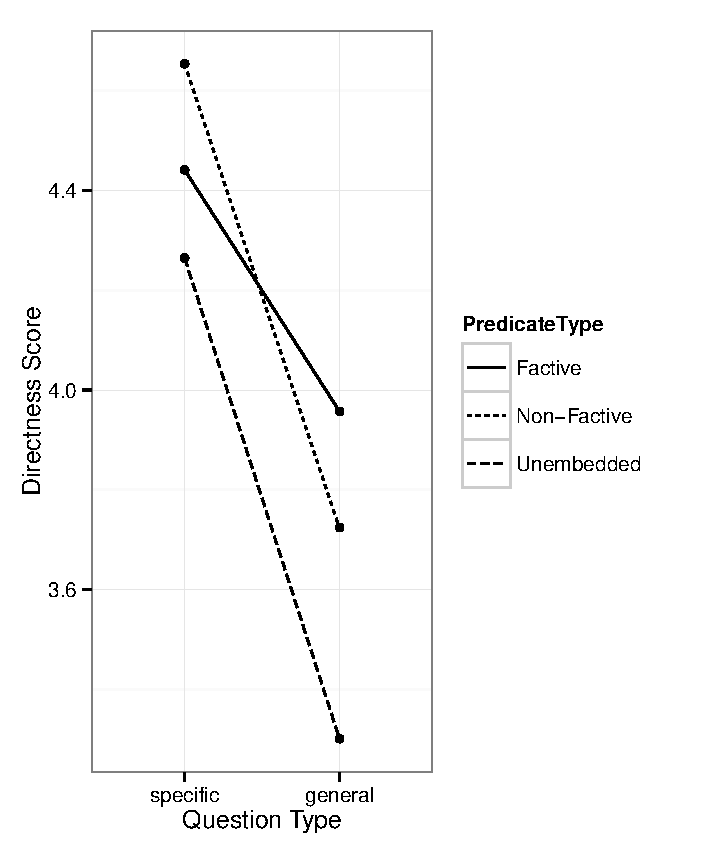
\includegraphics[scale=0.8]{figures/LinePlotNonColour.pdf}
\caption{Directness ratings in Experiment 1 by question type (general vs.\ specific) and response type (factive vs.\ non-factive vs.\ unembedded)}
\label{fig:ev2:englishStudy}
\end{figure} 

Given that discourse contexts can be manipulated such that factives\is{factive} do appear to license MPU\is{Main Point of Utterance}, the next experiment tests whether a discourse context manipulation that shifts MPU\is{Main Point of Utterance} can also influence the acceptability of EV2 in \ili{Swedish}.


\section{Experiment 2: Swedish embedded V2}

Acceptability judgments were elicited from native \ili{Swedish} speakers in a 4 $\times$ 2 $\times$ 2 design that manipulated MPU\is{Main Point of Utterance} (main vs.\ embedded clause), verb class (communicative assertive, epistemic assertive, (emotive) \isi{factive}, (cognitive) semifactive),  and word order (EV2 vs.\ EV3).\footnote{In order to keep the questionnaire to a manageable length, we did not include examples of Class C predicates (e.g.\ \textit{deny}, \textit{doubt}, etc).}
 Since the consensus among researchers appears to be that EV2 is optional even when it is permitted, EV3 word order is predicted to be generally more acceptable than EV2.  If MPU\is{Main Point of Utterance} is lexically defined, we predict a word order $\times$ predicate class interaction whereby EV2 is acceptable only under assertives and under semifactives (see \citealt{WiklundEtAl2009}).  Alternatively, if MPU\is{Main Point of Utterance} is a property of utterances in context, we predict a word order $\times$ MPU\is{Main Point of Utterance} interaction whereby EV2 is more acceptable when the context signals that the embedded clause is the MPU\is{Main Point of Utterance} (see \citealt{JensenChristensen2013}).

\subsection{Methodology}

\subsubsection{Participants}
%\noindent \textit{Participants}

A group of 118 \ili{Swedish}-speaking students (age 18--19) from a senior high school in the northern \ili{Swedish} city of Ume{\aa} participated in the study. All participants were volunteers.

\subsubsection{Materials}
%noindent \textit{Materials}

Each item consisted of a 3-\isi{utterance} passage.  For the 16 experimental items, these passages contained a background sentence, a \isi{question} to establish MPU\is{Main Point of Utterance} for the target sentence, and the target sentence itself, as in (\ref{ex:expt2-materials}).  The background sentence introduced two individuals. The second \isi{utterance} posed a \isi{question} about one of those two individuals.  The target sentence mentioned one individual as the subject of the matrix clause and one as the subject of the embedded clause.  

The MPU\is{Main Point of Utterance} manipulation was achieved via the combination of the \isi{question} posed and the positions of mention of the two individuals in the target sentence.  In (\ref{ex:expt2-materials}), the target sentence mentions Carina as the matrix clause subject and Albin as the embedded clause subject.  The \isi{question} to trigger main clause MPU\is{Main Point of Utterance} therefore asks about Carina; the embedded clause MPU\is{Main Point of Utterance} trigger asks about Albin.  The word order manipulation was indicated via the position of \isi{negation} relative to the verb.  Both MPU\is{Main Point of Utterance} and word order were manipulated within items.  With this design, each passage could be minimally varied to construct 4 conditions (MPU-matrix:EV2, MPU-embedded:EV2, MPU-matrix:EV3, MPU-embedded:EV3).  

\protectedex{
	\ea\label{ex:expt2-materials}\begin{itemize}
		\item[] \textbf{Background}: \\ 
		Lille Albin och hans mamma Carina gick och s{\aa}g en film p{\aa} bio. \\ 
		`Little Albin and his mother Carina went to see a movie in the cinema.'
		\item[] \textbf{Embedded Clause MPU\is{Main Point of Utterance} Trigger}:\\ 
		Hur upplevde Albin biobes\"oket?\\ 
		`How did Albin find the visit to the cinema?' 
		\item[] \textbf{Main Clause MPU\is{Main Point of Utterance} Trigger}:  \\ 
		Hur upplevde  Carina biobes\"oket? \\ 
		`How did Carina find the visit to the cinema?'
		\item[] \textbf{Target}: 

		\gll Carina gissade att han (\textbf{hade}) nog inte (\textbf{hade}) v\"antat sig s{\aa} mycket action.\\
		Carina guessed that he (had) maybe not (had) expected self so much action\\
		\glt `Carina guessed that he probably hadn't expected that much action.'
	\end{itemize} \z }
%\begin{exe}
%\ex \label{expt2:materials}\begin{itemize}
%\item[] \textbf{Background}: \\ 
%Lille Albin och hans mamma Carina gick och s{\aa}g en film p{\aa} bio. \\ 
%`Little Albin and his mother Carina went to see a movie in the cinema.'
%\item[] \textbf{Embedded Clause MPU\is{Main Point of Utterance} Trigger}:\\ 
%Hur upplevde Albin biobes\"oket?\\ 
%`How did Albin find the visit to the cinema?' 
%\item[] \textbf{Main Clause MPU\is{Main Point of Utterance} Trigger}:  \\ 
%Hur upplevde  Carina biobes\"oket? \\ 
%`How did Carina find the visit to the cinema?'
%\item[] \textbf{Target}: 
%\gll Carina gissade att han (\textbf{hade}) nog inte (\textbf{hade}) v\"antat sig s{\aa} mycket action.\\
%Carina guessed that he (had) maybe not (had) expected self so much action.\\
%\trans `Carina guessed that he probably hadn't expected that much action.'
%\end{itemize}
%\end{exe}


The remaining manipulation of predicate class of the embedding verb was between items (4 items for each of 4 predicate classes).  The predicates were classified according to \citeauthor{HooperThompson1973}'s scheme, omitting their Class C: (communicative) assertive, (epistemic) assertive, \isi{factive} (emotive), semifactive
(cognitive).\footnote{Communicative and epistemic assertives are sometimes labeled ``weak'' and ``strong'' assertive \citet{WiklundEtAl2009}. However, it is not at all clear to us that strength of \isi{assertion}, in any straightforward understanding of the concept, is the relevant variable: rather the verbs in Class A are verbs of communication, while those in Class B are verbs of thought or cognition.} The predicates we used for each group are listed in \tabref{tab:ev2:embverbs}. 

% \todo{is semelfactive intended?}
\begin{table}%[H]
%\renewcommand{\arraystretch}{1.4}
%\begin{center}
  %{\small 
  	\begin{tabular}{ c   l  l  l  l  l } %\midrule 
  		\lsptoprule	
					& \textbf{Assertive} 	& \textbf{Assertive} 	& \textbf{Factive} 				& \textbf{Semifactive} \\ %\midrule 
					& \textbf{(communicative)} 	& \textbf{(Epistemic)} 	& \textbf{} 				& \textbf{} \\ %\midrule 
		\midrule			
 \textbf{Group 1}  	& \textit{s\"aga} 						&  \textit{anta}  					& \textit{vara l\"attad}		& \textit{uppt\"acka}   \\ 
 			& say 									& suppose 							& be relieved 					& discover \\ \midrule
 \textbf{Group 2} 	& \textit{ber\"atta}  					& \textit{f\"ormoda}  				& \textit{vara glad}  			&  \textit{m\"arka}   \\ 
 			& tell 									& assume 							& be happy 						& notice \\ \midrule
 \textbf{Group 3}  	& \textit{f\"orklara}  					& \textit{gissa}   					& \textit{vara ledsen}  		& \textit{komma fram till }  \\ 
  		& explain 								& guess 							& be sad/sorry 					& arrive at \\ \midrule
 \textbf{Group 4}  	& \textit{h\"avda}  					& \textit{vara s\"aker} 	 		& \textit{vara f\"orv{\aa}nad}  & \textit{f{\aa} veta}  \\ 
 		& claim 								& be sure 							& be surprised 					& come to know \\ 
		\lspbottomrule 
  \end{tabular}
  %}
%\end{center}
\caption{The clause-embedding predicates used in the experiment, by predicate-type.}
\label{tab:ev2:embverbs}  
\end{table}



The experiment consisted of 16 experimental items mixed with 16 fillers. Fillers consisted of passages in the same 3-\isi{utterance} format and their complexity roughly matched the experimental items, with embedded complement clauses and \isi{relative} clauses. The fillers varied as to whether they were fully grammatical (n=8), fully ungrammatical (n=4), or pragmatically infelicitous (n=4).  

So as not to repeat verbs across items, only 16 experimental items were constructed.  Each participant saw all 16 items and therefore saw each of the 16 conditions only once.  Because of this, a large number of participants were recruited.  The 16 experimental items were assigned to conditions in a \ili{Latin} Square design such that, across 4 lists, each item was presented in each MPU\is{Main Point of Utterance} $\times$ word order condition once and each participant saw each condition once.

\subsubsection{Procedure}
%\noindent \textit{Procedure}

The experiment was conducted as a pen and paper task in a classroom setting.
The experimenter provided participants with a booklet containing the
instructions and passages (all in \ili{Swedish}).  Participants were instructed to
judge the acceptability of the passages on a scale from 1 to 6, where 1
represented \textbf{unacceptable}, and 6 represented \textbf{fully acceptable}.
Each passage appeared on a page by itself with a {question} asking participants to ``Indicate how natural you consider the answers to the questions to be."  The task took roughly 20 minutes.

\subsubsection{Analysis}
%\noindent \textit{Analysis}


The raw scores were analyzed with linear mixed effects models in R, with
participants and items as random effects.  Maximum random effect structure was
used \citep{BarrEtAl2013}.  The word order and MPU\is{Main Point of Utterance} conditions were centered, and 
predicate class was contrast coded.  We conducted likelihood-ratio tests
between mixed-effects models differing only in the presence or absence of a
fixed main effect or interaction.  We report the p-values derived from the model
comparisons.

\subsection{Results}
Judgments from 6 non-native \ili{Swedish} speakers were removed.  In addition, 8 participants whose judgments failed to distinguish the grammatical and ungrammatical fillers were excluded.  20 requested judgments (1\%) were left blank. The remaining dataset consisted of 1644 judgments on experimental items from 104 native speakers.

The results from Experiment 2 are illustrated in \figref{fig:ev2:swedishStudy}.  As predicted, EV3 receiving higher ratings than EV2 (main effect of word order:  p$<$0.001).  In addition, higher ratings were assigned to passages that contained semifactive and communicative assertive embedding verbs (main effect of predicate class: p$<$0.001). This main effect of predicate class was driven by a word order $\times$ predicate class interaction (p$<$0.001): As predicted under an account in which MPU\is{Main Point of Utterance} is lexically defined and the embedding verb directly influences the acceptability of EV2, ratings for EV2 were almost as high as for EV3 for the class of communicative assertives and the class of semifactives.  There was no main effect of MPU\is{Main Point of Utterance} (p=0.88), and contrary to a context-driven account of the role of MPU\is{Main Point of Utterance} in EV2, there was no interaction with MPU\is{Main Point of Utterance} (p's$>$0.75).

Given \citeauthor{Julien2009}´s claim that -- regardless of the MPU\is{Main Point of Utterance} -- a speaker can use EV2 when reporting a 3rd party's \isi{assertion}, and the higher frequency of EV2  reported by Jensen \& Christensen for communicative assertives over epistemic assertives in their \ili{Danish} corpus, we tested whether the acceptability of EV2 is higher for communicative assertives than epistemic assertives. A model of the data across those two predicate classes shows a word order $\times$ predicate class interaction (p$<$0.001) whereby the acceptability of EV2 is indeed much higher for communicative assertives than epistemic assertives.  This interaction appears alongside a main effect of word order (p$<$0.001), a main effect of predicate class (p$<$0.001) and non-significant effects and interactions for MPU\is{Main Point of Utterance} (p's$>$0.68). This result, which matches the frequencies of EV2 in \ili{Danish} reported by \citeauthor{JensenChristensen2013}, lends support to \citeauthor{Julien2009}´s claim.

\begin{figure}
% \centering
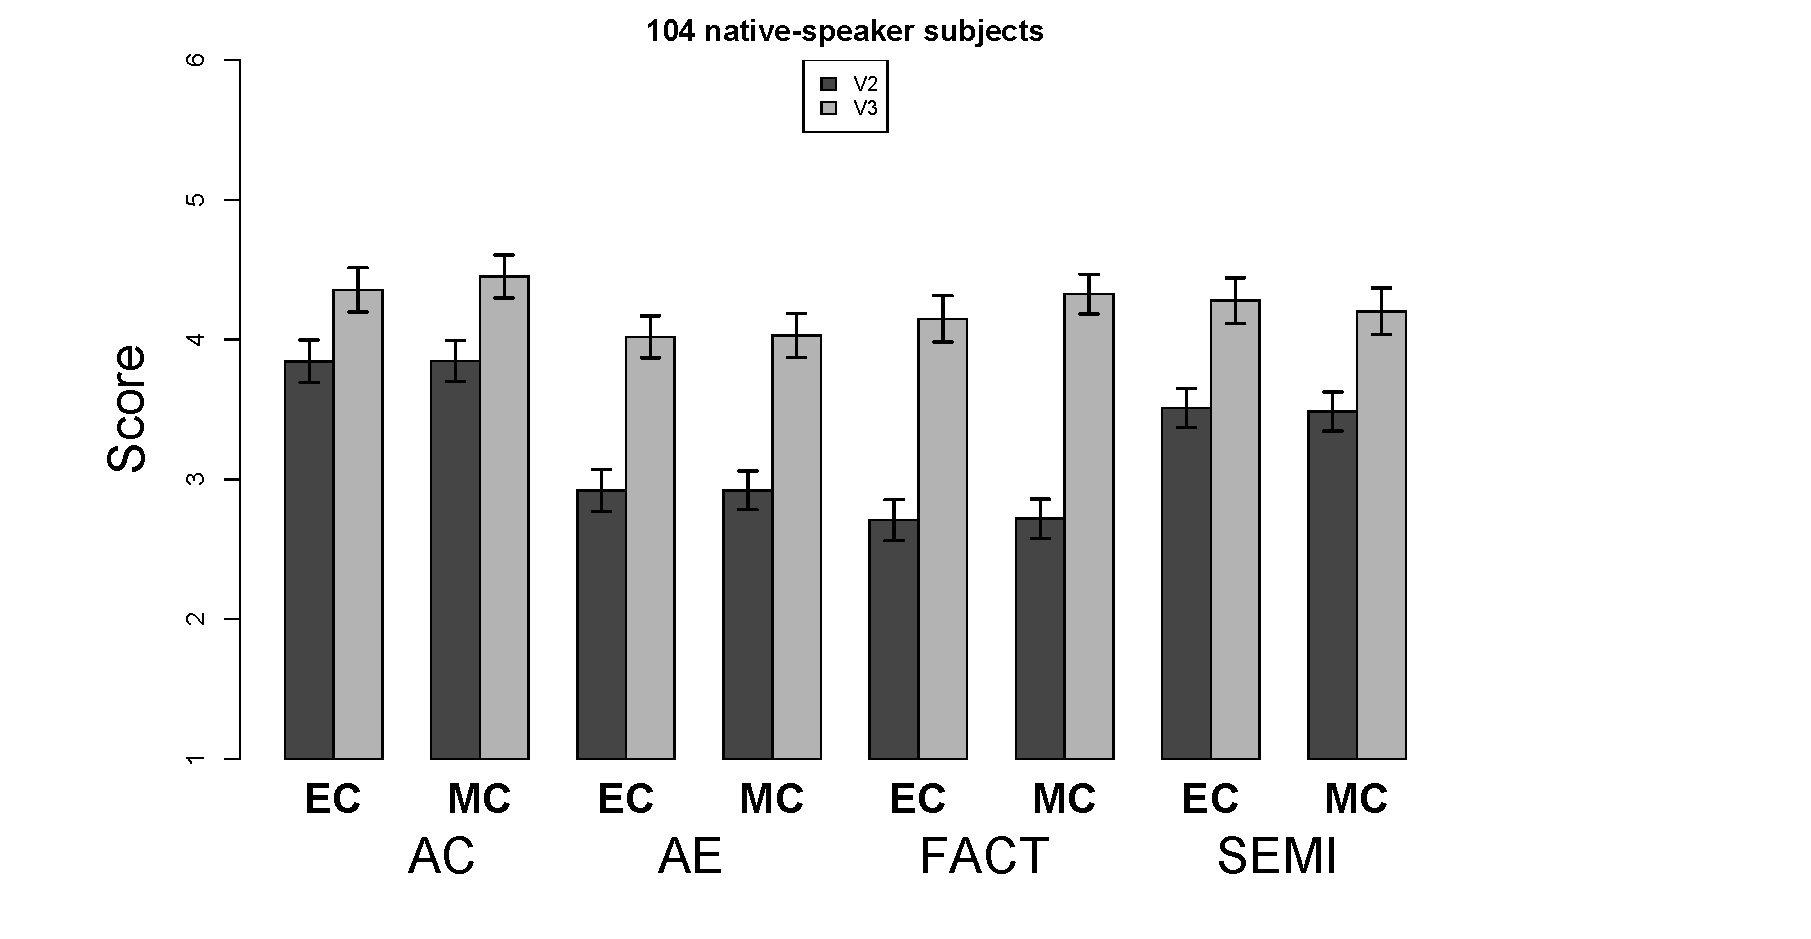
\includegraphics[width=\textwidth]{figures/EV2graph104subj.pdf}
\caption{Acceptability judgments of target sentences in Experiment 2, broken down by MPU (Main Clause (MC), Embedded Clause (EC)),  Predicate Class (communicative assertive (AC), epistemic assertive (AE), factive (FACT), semifactive (SEMI)), and Word Order (V2, V3).}
\label{fig:ev2:swedishStudy}
\end{figure}

These results support the claim that \ili{Swedish} EV2 is possible under semi-\isi{factive} (\textit{discover/realize}) and non-\isi{factive} (\textit{think/claim}) clause-embedding predicates, but not under purely \isi{factive} ones (\textit{be happy/be surprised}) (\citealt{WiklundEtAl2009}).    However, the results show no interaction between word order and MPU\is{Main Point of Utterance}. That is, our data suggest, contra \citet{JensenChristensen2013}, that the low acceptability of V2\is{verb second} under factives\is{factive} cannot be explained by the twin hypotheses that MPU\is{Main Point of Utterance} licenses EV2 and that factives\is{factive} cannot embed MPU\is{Main Point of Utterance}.  Even if we set aside the factives\is{factive}, there was no effect of MPU\is{Main Point of Utterance} when the embedding predicate was a non-\isi{factive} or a semi-\isi{factive}. There is no controversy in the literature about the ability of these predicates to embed the MPU\is{Main Point of Utterance}. But even in these contexts, participants did not rate the use of EV2 any higher in the embedded-MPU\is{Main Point of Utterance} condition.  Our results therefore suggest that MPU\is{Main Point of Utterance} is not relevant, and a different account is needed to explain the unavailability of EV2 under factives\is{factive}.

\section{Discussion and conclusion}

In this paper we have described two experiments that bear on the relation between ``\isi{assertion},'' factivity, and the distribution of one classic case of an embedded root phenomenon: embedded Verb Second (EV2) in \ili{Swedish}. As discussed in Section~\ref{sec:factivity}, although \citet{HooperThompson1973}  classified complement clauses licensing or disallowing \isi{root phenomena} in terms of the semantic\is{semantics} properties of the embedding predicates, and the lexical classes that they set up have been extensively referred to in the subsequent literature, their explanation for the effect of these embedding predicates was a functional/\isi{pragmatic} one. For example, factives\is{factive} were argued to disallow \isi{root phenomena} in their complements because their complements were presupposed, and hence could not be \textbf{asserted}. Indeed, H\&T argued that even predicates in classes that allow embedded \isi{root phenomena} only do so when their complement is in fact the ``main \isi{assertion}'' of the \isi{utterance}, and the embedding predicate is being used parenthetically -- see for example their discussion of the contrast between (\ref{ex:thatnever}a) and (\ref{ex:thatnever}b), their (67) and (68).% p. 476

\protectedex{
	\ea \label{ex:thatnever}
	\langinfo{}{}{\citealt[476]{HooperThompson1973}}

		\ea *That never in his life has he had to {borrow} money is true.
		\ex It's true that never in his life has he had to {borrow} money.
        \z
	\z }

%\begin{exe}
%	\ex \begin{xlist}
%		\ex[*]{That never in his life has he had to \isi{borrow} money is true.}\label{thatnever}
%		\ex[]{It's true that never in his life has he had to \isi{borrow} money.}\label{itstrue}
%	\end{xlist} 
%\end{exe}

\noindent In their recent corpus work, \citet{JensenChristensen2013} have essentially adopted this explanation for the distribution of EV2 in \ili{Danish}.

As discussed in the same section, the work of \citet{Simons2007} has provided a way to 
test whether indeed the effect of the embedding predicate is only epiphenomenal, as argued by \citeauthor{JensenChristensen2013}, since we should be able to manipulate MPU\is{Main Point of Utterance} independently of the class of the embedding predicate. 
In Experiment 1 we tested \citeauthor{Simons2007}' claim that factives\is{factive} can be used parenthetically.  As reported in Section~\ref{sec:exp1}, our experiment supports Simons' claim.   First, the contrast in participants' judgments on the directness of the answer depending on the \isi{question} type shows that we were successful in manipulating the discourse context to change what they took to be the MPU\is{Main Point of Utterance}. Second, the fact that participants readily judged the complements of factives\is{factive} to constitute direct answers, in the relevant context, bears out Simons' view that factives\is{factive} need not necessarily resist ``\isi{assertion}'': that is, in the right context, factives\is{factive} \textit{can} indeed embed MPU\is{Main Point of Utterance} clauses.

Having established that participants can show sensitivity to the experimental manipulation of the MPU\is{Main Point of Utterance} by a preceding \isi{question}, and that factives\is{factive} can embed the MPU\is{Main Point of Utterance}, in Experiment 2 we then tested whether the same type of manipulation of the MPU\is{Main Point of Utterance} affects the acceptability of EV2 in \ili{Swedish}. 
%That is,
%Experiment 2 then tested whether this sensitivity to MPU\is{Main Point of Utterance} can be transferred over to EV2 contexts in \ili{Swedish}:  
%if a \isi{pragmatic} context can be established that targets an embedded clause as the MPU\is{Main Point of Utterance}, is EV2 licensed, or is the acceptability of EV2 dependent directly on predicate class, regardless of the location of the MPU\is{Main Point of Utterance}? 
 In contrast to the robust effects of MPU\is{Main Point of Utterance} in Experiment 1, the MPU\is{Main Point of Utterance} manipulations in Experiment 2 yielded no differences in the acceptability of EV2.  Rather, the acceptability of EV2 was shown to be driven entirely by predicate class.  EV2 was most acceptable for semifactives and communicative assertives.  Compared with assertive predicates that explicitly convey a communicative act, epistemic (or cognitive) assertives yielded much lower ratings for EV2.  And finally, EV2 was least acceptable under factives\is{factive}.  These EV2 preferences match the data reported by \citeauthor{JensenChristensen2013} and \citeauthor{WiklundEtAl2009}, but an account of such data that relies on MPU\is{Main Point of Utterance} was not supported.  Lastly, we observed an overall preference for EV3 across all predicate classes. This is in keeping with prior work suggesting that EV2, even when permitted, is never required. 

These results clearly raise the \isi{question}: if the deeper explanation for the effect of the different predicates is not a correlation with MPU\is{Main Point of Utterance}, what is the alternative?
%
%Experiment 1 was designed to test whether the status of a clause as the Main Point of Utterance\is{utterance} affects the availability of EV2, as measured by acceptability judgments of native speakers looking at utterances in context. As we have just discussed, we found no evidence in favour of this hypothesis. Regardless of the class of the embedding verb, manipulating the context so that the embedded clause was or was not the MPU\is{Main Point of Utterance} had no effect. On the other hand, participants did reliably distinguish between the complements of different classes of embedding verbs. This evidently raises the \isi{question}: if MPU\is{Main Point of Utterance} status is not what licenses EV2, what does?
The proposal in \citet{WiklundEtAl2009} is that certain classes of verb (H\&T's Classes A, B, and E -- the ``strongly and weakly assertive'' predicates and the semifactives) syntactically select for a particular ``size'' of complement clause (specifically ForceP), while the other classes (C and D, the non-assertive, non-presuppositional predicates, and the factives\is{factive}) select a smaller clausal constituent that lacks this \isi{projection}; V2\is{verb second} is syntactically possible within ForceP but not in the smaller structure.  A variant of this kind of account would be to adopt the ``intervention'' approach put forward in \citet{Haegeman2010,Haegeman2012MCP}, among other works, according to which A$'$-movement inside clauses may be blocked by other (often covert) operations of A$'$-movement. Thus for example Haegeman argues that English argument topicalisation inside conditionals is blocked by the A$'$-movement of a world operator; similarly, factives\is{factive} have been argued to involve movement of a \isi{factive} operator, which would also interfere with other A$'$ movement (see for example \citealt{ZanuttiniPortner2003}). If we were to assume that V2\is{verb second} always involves A$'$-movement of some phrase to the left periphery (in the examples we have been citing, this is always the subject, but its high position is evidenced indirectly by the high position of the verb, to the left of \isi{negation}), this type of account gives an essentially syntactic explanation\largerpage for the low acceptability of V2\is{verb second} in the complement to factives\is{factive} that we observed in our data. %REPLACED: Thus for example Haegeman argues that English argument topicalisation inside conditionals is blocked by the A$'$-movement of a world operator; similarly, factives\is{factive} have been argued to involve movement of a \isi{factive} operator, which would also interfere with other A$'$ movement (see for example \citealt{zanuttini-portner03}).  On the assumption that V2\is{verb second} always involves A$'$-movement of some phrase to the left periphery (in the examples we have been citing, this is always the subject, but its high position is evidenced indirectly by the high position of the verb, to the left of \isi{negation}), this type of account gives an essentially syntactic explanation for the low acceptability of V2\is{verb second} in the complement to factives\is{factive} that we observed in our data.

What prevents such accounts from being circular is that the smaller clause size (in a ``truncation'' account such as the one sketched in \citealt{WiklundEtAl2009}) or the operator movement (in an intervention account along the lines of \citealt{ZanuttiniPortner2003,Haegeman2010,Haegeman2012MCP}) has semantic\is{semantics}/\isi{pragmatic} effects.  \citeauthor{WiklundEtAl2009}  propose that ``MPU\is{Main Point of Utterance} and the possibility of non-subject-topicalization (including unrestricted V2\is{verb second}) are licensed by the same structural domain [...], ForceP''; \citeauthor{ZanuttiniPortner2003} derive the \isi{factive} interpretation from the presence of the \isi{factive} operator.  

But the results of Experiment 2 are problematic for both of these variants, for different reasons. Taking the clause-truncation explanation first: as discussed above in \sectref{nonfactivityOrMPU}, and as suggested by the quote just above, \citeauthor{WiklundEtAl2009} appear to take the view that factives\is{factive} (for example) cannot embed the MPU\is{Main Point of Utterance}. But as argued by \citeauthor{Simons2007}, and now supported also by the results of Experiment 1, it appears that speakers \textit{are} able to treat the complement of a \isi{factive} as the MPU\is{Main Point of Utterance}.  Nevertheless, Experiment 2 showed that EV2 is always given low ratings in the complements of factives\is{factive} -- \textit{even when the context sets this up as the MPU}.  In consequence, the analysis sketched in \citet{WiklundEtAl2009} does not in fact avoid a circular account of possible environments for EV2. The independent evidence for the distribution of ForceP -- the syntactic environment in which V2\is{verb second} is licensed, by hypothesis -- was to be the possibility for an MPU\is{Main Point of Utterance} interpretation. But as we have just seen, MPU\is{Main Point of Utterance} interpretation \textit{is} possible for the complement of factives\is{factive}, but our results show that this is not an environment in which speakers accept EV2.  So now it appears to be just a lexical idiosyncrasy that factives\is{factive} do not readily license EV2 in their complements.

Our results are also problematic for an intervention approach to the blocking effect of factivity. Here the problem is the finding that semifactives constitute one of the most favourable environments for EV2. This finding confirms what has already been claimed on the basis of speaker judgments and corpus work (e.g. \citealt{WiklundEtAl2009,JensenChristensen2013,Julien2015}) and what H\&T observed for embedded \isi{root phenomena} in English. But if factivity is the result of the presence of a \isi{factive} operator,  this operator ought also to be present in the complement to semi-factives\is{factive} in those environments in which the \isi{factive} interpretation is not cancelled -- and all the semifactive environments in our experiment were of this type (declarative non-\is{Modal}modal sentences).  Clearly a better understanding of the exact nature of the distinction between factives\is{factive} and semifactives is crucial here, and this is one topic that merits future investigation.

A sceptical reader may wonder whether the participants in Experiment 2 were paying sufficient attention to the discourse context manipulation and, if they were, whether the manipulation successfully established embedded MPU\is{Main Point of Utterance} interpretations.  We know from the first study that participants in experimental paradigms like this are capable of attending to the discourse context in evaluating a target sentence.  However, the relationship between the two paradigms is indirect -- in Experiment 1, the task asks participants to pay attention to how the target sentence responds to the posed \isi{question}, whereas in Experiment 2, the task asks for an acceptability judgment.  The tasks differ because Experiment 1 was probing factivity and MPU\is{Main Point of Utterance}, whereas Experiment 2 was designed to determine the status of EV2 across different contexts.   If participants in Experiment 2 effectively ignored the \isi{question} context, then it might still be possible to give an explanation for the effect of verb class on the acceptability of EV2 that appeals to MPU\is{Main Point of Utterance} as a crucial factor. For example, since it is at least plausible that the frequency of embedded MPU\is{Main Point of Utterance} in the complement of factives\is{factive} is low compared to its occurrence in other contexts, it could be that speakers draw on this knowledge when assessing the acceptability of sentences considered out of context. 
Finding a single task that could overcome this potential problem is tricky, but future work should look to address the indirect relationship between the two experiments just described, perhaps by including in the acceptability ratings a measure of participants' assessment of a target sentence as an appropriate answer to the posed \isi{question}.


\section*{Acknowledgments} 

Thanks to participants at the Experimental Study of Meaning Lab at the University of Pennsylvania for helpful feedback and comments. Likewise to audiences at MACSIM V at the University of Delaware, CSI Lisbon (2014), LEL Syntax and Semantics seminar at the University of Edinburgh, and the ULAB/LEL undergraduate conferences. Thanks to Hezekiah Akiva Bacovcin for help with the statistical analysis of Experiment 1 and to research assistant Ivana \v{Z}etko for help with data processing for Experiment 2. Particular thanks to Florian Schwarz for guidance, feedback, and help with statistical analysis of Experiment 1. Part of this work was supported by NSF grant BCS-1349009 to Florian Schwarz.

Like so much work on the syntax of {Scandinavian}, the inspiration for this study can be traced back to Anders Holmberg’s research (going all the way back to his dissertation, in fact).  We are grateful to have the opportunity to contribute to this volume in his honour.
	
{\sloppy
\printbibliography[heading=subbibliography,notkeyword=this]
}

\end{document}
